\section{Marco Teórico}
En la sociedad actual, la tecnología se ha convertido en un medio importante dentro de la educación para apoyar los procesos de aprendizaje de los individuos. Por ello, se han creado aplicaciones que facilitan este proceso, como por ejemplo, los objetos virtuales de Aprendizaje \cite{Tovar2014}. Según lo señalado por Moral y Cernea \cite{DelMoral2005} estos: “deben hacer uso de la narrativa hipermedial para que establezca relaciones que complementen la información a través de enlaces y mapas conceptuales que presenten la información de una manera sintética y estructurada, priorizando la internavegabilidad” .

A raíz de lo anterior, se puede observar como otra alternativa para apoyar los procesos de aprendizaje los sistemas hipermedia. No obstante, al ser estos sistemas “estáticos”, es decir, que proporcionan el mismo contenido de página y el mismo conjunto de enlaces a todos los usuarios -sin tener en cuenta, las diferentes motivaciones, personalidades, conocimientos y experiencias de los mismos-, limitan la capacidad de ayuda en este proceso, por tal razón, se hace necesario extender las funciones de estos sistemas y es ahí donde se introduce el tema de sistema hipermedia adaptativo \cite{kubes2007}.

En este sentido, para el desarrollo del presente proyecto, se tomará como marco teórico algunos referentes en: sistema hipermedia, objetos virtuales de aprendizaje, estilos cognitivos, metodología Methadis para el diseño de sistemas hipermedia adaptativos y metodología Extreme Programming, ya que son temas específicos que permiten contextualizar la problemática tratada.

\subsection{Sistema Hipermedia}
Un sistema hipermedia es una aplicación con características hipermediales e hipertextuales \cite{Jose2004}, es decir, son aplicaciones donde la información se encuentra en forma de texto, imágenes y sonido, y a su vez están conectadas entre sí, lo que permite al usuario navegar entre ellos mediante enlaces.

Los componentes principales de un sistema hipermedia son \cite{Vrasidas2002}: 

\begin{itemize}
    \item \textbf{Los nodos:} Son los elementos principales de la información, puede ser texto, vídeo, sonido o imágenes. 
    \item \textbf{Enlaces:} Permiten al usuario moverse de un nodo a otro con el objetivo de poder acceder a la información que contienen estos. 
\end{itemize}

\begin{figure}[H]
    \centering
    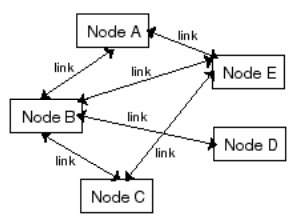
\includegraphics[scale=0.6]{Capitulo_2/2_MarcoTeorico/imagenes/d1.png}
    \caption{Componentes hipermedia}
    \scriptsize \textbf{Fuente:} \cite{Vrasidas2002}
    \label{fig:componentesHipermedia}
\end{figure}


\textbf{Ventajas y desventajas de los sistemas hipermedias \cite{Jose2004}.} 
Una de las principales ventajas de estos sistemas es su estructura en forma de red, ya que modela las teorías del funcionamiento asociativo del cerebro simulando así la organización de la mente humana, lo cual permite que sea más comprensible y fácil de usar, asimismo, permite que el usuario controle lo qué quiere ver y cuándo lo quiere ver.


Lo anterior, ha hecho que estos sistemas sean de gran utilidad para diferentes áreas: sociales, comerciales, educativas, entre otras. En el ámbito educativo se hacer uso para mejorar el proceso de aprendizaje, permitiendo así que este sea más interactivo. 


No obstante, entre sus desventajas está la posible existencia de sobrecarga cognitiva para sus usuarios. Esto debido a la cantidad de caminos que este puede tomar, ocasionando la posible pérdida dentro de la aplicación y la incapacidad para identificar donde se encuentra dentro de la misma. A raíz de esto, para mejorar la usabilidad surgen los sistemas hipermedia adaptativos \cite{Medina2002}, cuyas características son iguales a la de los sistemas hipermedia, con el agregado de que se adaptan al usuario.


\subsubsection{Sistema Hipermedia Adaptativo}
Brusilovsky define un sistema hipermedia adaptativo como: “Todos los sistemas de hipermedia e hipertexto que reflejan algunas de las características del usuario en un perfil de usuario, y utilizan este perfil para adaptar varios aspectos visibles del sistema al usuario \cite{Brusilovsky1998}.  

Dicho en otras palabras, un sistema hipermedia adaptativo es aquel que cuenta con los siguientes tres criterios \cite{Brusilovsky1996} :

\begin{itemize}
     \item Debe ser un sistema de hipertexto o hipermedia.
     
     \item Debe tener un modelo de usuario.
     
     \item Debe ser capaz de adaptar la hipermedia utilizando este modelo.
\end{itemize}
\ \\
\textbf{Componentes de un sistema hipermedia adaptativo} \cite{Graf2007}\ \\
Los componentes básicos de un Sistema Hipermedia Adaptativo son:
\ \\
\begin{itemize}
    \item \textbf{Modelo del dominio:} Describe la estructura del contenido de la información de la aplicación. Está compuesto por conceptos y las relaciones entre ellos. Generalmente, los conceptos están relacionados entre sí, por lo tanto, la estructura del contenido forma una especie de red semántica.
    
    \item \textbf{Modelo de usuario:} Suministra información de las preferencias, características, intereses e interacciones que el usuario realiza en el sistema. Esta información se utiliza para que el sistema se adapte adecuadamente. 

    Existen diferentes maneras en las que puede llevar acabo el modelado de usuario. Una de ellas es que se puede realizar de forma automática o involucrando al usuario en el proceso. De forma automática se basa en el comportamiento y las acciones de los usuarios cuando están utilizando el sistema para el aprendizaje, mientras que, si se involucra al usuario en el proceso de construcción del modelo de usuario, este debe proporcionar información explícita para poder construirlo, por ejemplo, responder un cuestionario con el fin de obtener información sobre ellos.
    
    Otra manera de llevar acabo el modelado del usuario es de forma estática o dinámica. Estática solo se realiza una vez y casi siempre al inicio del registro de usuarios y, dinámica, se puede realizar varias veces ya que el modelo de usuario está constantemente actualizándose.
    
    \item \textbf{Modelo de adaptación:} Consiste en adecuar y modificar los contenidos con base en la información obtenida en el modelo del usuario.

\end{itemize}

\ \\
\textbf{Métodos de adaptación} \cite{Brusilovsky1996} \ \\
Como ya se mencionó, la adaptación de los sistemas hipermedia se basa en las características del usuario, esta adaptación se puede dar en los dos elementos que forman la estructura del sistema: en los nodos de información o en los enlaces que hay entre los nodos del sistema. Por lo tanto, los métodos de adaptación que se puede encontrar un sistema hipermedia son:

\begin{itemize}
    \item Adaptación de nivel de contenido o presentación adaptativa: Forma en que se presentan los contenidos (adaptación de texto y adaptación de multimedia).

\item Adaptación de nivel de enlace o soporte de navegación adaptativa: Forma en que se presentan los enlaces (ocultación de enlaces, clasificación, anotación, guía directa y adaptación de mapas de hipertexto).

\end{itemize}
Cabe anotar que un sistema hipermedia adaptativo puede poseer una de estas adaptaciones o simultáneamente ambas.


\subsubsection{Sistemas Hipermedia Adaptativos en la educación}
La educación se ha convertido en una de las áreas de aplicación más populares de en la investigación y prueba de los sistemas hipermedia adaptativos, esto debido a que no todos los usuarios (estudiantes) tienen los mismos niveles de conocimiento y estrategias de aprendizaje \cite{Brusilovsky1996} . 
	
Las primeras investigaciones sobre los sistemas adaptativos en la educación se enfocaron en los Sistemas Tutoriales Inteligentes (ITS). Los primeros ITS proporcionaban poco material de aprendizaje, ya que se asumía que el conocimiento requerido del usuario se debería de adquirir fuera del sistema. Sin embargo, con el auge de las capacidades informáticas, los desarrolladores de los ITS consideraron razonable proporcionarles a estos, materiales de aprendizaje en formato de hipertexto o multimedia. Esta combinación de ITS con material de aprendizaje hipermedia fue el inicio para la investigación de los sistemas hipermedia adaptativos en la educación. 

Años más tarde con el apogeo de la Word Wide Web, se impulsó la investigación de los sistemas hipermedia adaptativo basados en la Web. Esta plataforma sirvió de laboratorio para que los investigadores exploraran nuevos métodos de adaptabilidad, por ejemplo \cite{Brusilovsky1999}:
\begin{itemize}
    \item El proyecto AHA! – Exploró varios enfoques para remover enlaces.
    \item	Metalinks – Exploró enfoques avanzados de estructuración hiperespacio.
    \item	INSPIRE – Exploró el uso de estilos de aprendizaje.
    \item	MANÍACO – Exploró enfoques innovadores para el modelado de usuario y presentación adaptativa. 
\end{itemize}

Así pues, los sistemas hipermedia adaptativos han demostrado una variedad de formas de integrar diversas técnicas de adaptación en los sistemas educativos basados en la Web. 
